\chapter{Implementazione}

\section{Specifiche di implementazione Java}

Riportiamo di seguito le classi Java utilizzate, con la loro suddivisione in package:

\begin{table}[!ht]
	\begin{tblr}{colspec=XX}
		\begin{minipage}[t]{0.45\textwidth}
			\paragraph{Package farmacia.boundary}
			\begin{itemize}[label=--]
				\item RegisterPage
				\item LoginPage
				\item HomePageCliente
				\item VisualizzaCatalogoPage
				\item FarmaciTableModel
				\item CreaOrdinePage
				\item VisualizzaStoricoOrdiniPage
				\item CercaFarmacoPage
				\item HomePageFarmacista
				\item AggiungiFarmacoPage
				\item ModificaFarmacoPage
				\item EliminaFarmacoPage
				\item VisualizzaCatalogoFarmacistaPage
				\item VisualizzaOrdiniClientiPage
				\item VisualizzaOrdiniAcquistoPage
				\item GeneraOrdineAcquistoPage
				\item ScegliFarmacoModificaPage
				\item RegistraRitiroOrdineClientePage
				\item RegistraConsegnaOrdineAcquistoPage
				\item HomePageDirettore
				\item GeneraReportPage
			\end{itemize}
		\end{minipage} &
		\begin{minipage}[t]{0.45\textwidth}
			\paragraph{Package farmacia.boundary.creaordine}
			\begin{itemize}[label=--]
				\item CreaOrdinePage
				\item OrdineTableModel
				\item OrdineTableColumnModel
				\item QuantitaCellEditor
			\end{itemize}

			\paragraph{Package farmacia.boundary.datepicker}
			\begin{itemize}[label=--]
				\item DatePanel
				\item DateTextField
			\end{itemize}

			\paragraph{Package farmacia.dto}
			\begin{itemize}[label=--]
				\item DTO
			\end{itemize}
		\end{minipage} \\
	\end{tblr}
\end{table}

\begin{table}[pt]
	\begin{tblr}{colspec=XX, rowsep=5pt}
		\begin{minipage}[t]{0.4\textwidth}
			\paragraph{Package farmacia.controller}
			\begin{itemize}[label=--]
				\item ControllerCatalogo
				\item ControllerOrdini
				\item ControllerUtenti
				\item ControllerReport
			\end{itemize}
		\end{minipage} &
		\begin{minipage}[t]{0.4\textwidth}
			\paragraph{farmacia.entity}
			\begin{itemize}[label=--]
				\item EntityCatalogo
				\item EntityCliente
				\item EntityUtente
				\item EntityFarmacia
				\item EntityFarmaco
				\item EntityOrdine
				\item EntityOrdineAcquisto
				\item Sessione
			\end{itemize}
		\end{minipage} \\
		\begin{minipage}[t]{0.4\textwidth}
			\paragraph{Package farmacia.database}
			\begin{itemize}[label=--]
				\item DBManager
				\item UtenteDAO
				\item FarmacoDAO
				\item OrdineDAO
				\item OrdineAcquistoDAO
			\end{itemize}
		\end{minipage} &
		\begin{minipage}[t]{0.4\textwidth}
			\paragraph{Package farmacia.exceptions}
			\begin{itemize}[label=--]
				\item DBException
				\item LoginFailedException
				\item RegistrationFailedException
				\item FarmacoCreationFailedException
				\item FarmacoNotFoundException
				\item OrderCreationFailedException
				\item OrderNotFoundException
				\item ReportException
			\end{itemize}
		\end{minipage} \\
		\begin{minipage}[t]{0.45\textwidth}
			\paragraph{Package farmacia.test.controllercatalogo}
			\begin{itemize}[label=--]
				\item AggiungiFarmacoTest
				\item CercaFarmacoTest
				\item CercaFarmacoInesistenteTest
				\item EliminaFarmacoTest
				\item ModificaFarmacoTest
				\item ModificaFarmacoInesistenteTest
			\end{itemize}
		\end{minipage} &
		\begin{minipage}[t]{0.4\textwidth}
			\paragraph{Package farmacia.test.controllerutenti}
			\begin{itemize}[label=--]
				\item LoginUtenteTest
				\item RegistraUtenteTest
			\end{itemize}
		\end{minipage} \\
		\begin{minipage}[t]{0.45\textwidth}
			\paragraph{Package farmacia.test.controllerordini}
			\begin{itemize}[label=--]
				\item CreaOrdineTest
				\item VisualizzaStoricoOrdiniTest
				\item AggiornaOrdineTest
				\item AggiornaOrdineAcquistoFarmaciaTest
				\item GeneraOrdineAcquistoFarmacistaTest
			\end{itemize}
		\end{minipage} &
		\begin{minipage}[t]{0.4\textwidth}
			\paragraph{Package farmacia.testcontrollerreport}
			\begin{itemize}[label=--]
				\item GeneraReportTest
			\end{itemize}
		\end{minipage} \\
		\begin{minipage}[t]{0.5\textwidth}
			\paragraph{Package farmacia}
			\begin{itemize}[label=--]
				\item Main
				\item TipoUtente
			\end{itemize}
		\end{minipage}
	\end{tblr}
\end{table}

\vfill
\pagebreak

Le linee di codice scritte sono:

\begin{itemize}[label=--]
	\item LOC = 6041
	\item LLOC = 4257
\end{itemize}

\section{Artefatti necessari per l'installazione e l'esecuzione}

Le dipendenze necessarie al fine di eseguire l'applicativo sono:
\begin{itemize}
	\item OpenJDK-22.0.1
	\item Oracle MySQL Server 8.0.38 (con il file db\_farmacia.sql)
	\item mysql-connector-j-8.4.0.jar
	% \item forms_rt.jar (libreria IntelliJ GUI Designer)
	\item junit-4.10.jar
	\item bluecatcode.junit.4.10.extended.jar (JUnit)
\end{itemize}

\section{Documentazione}

La documentazione del sistema è presente all'interno della cartella \texttt{javadoc/}.

\vfill
\pagebreak

\section{Diagramma di deployment}

\begin{figure}[h]
	\centering
	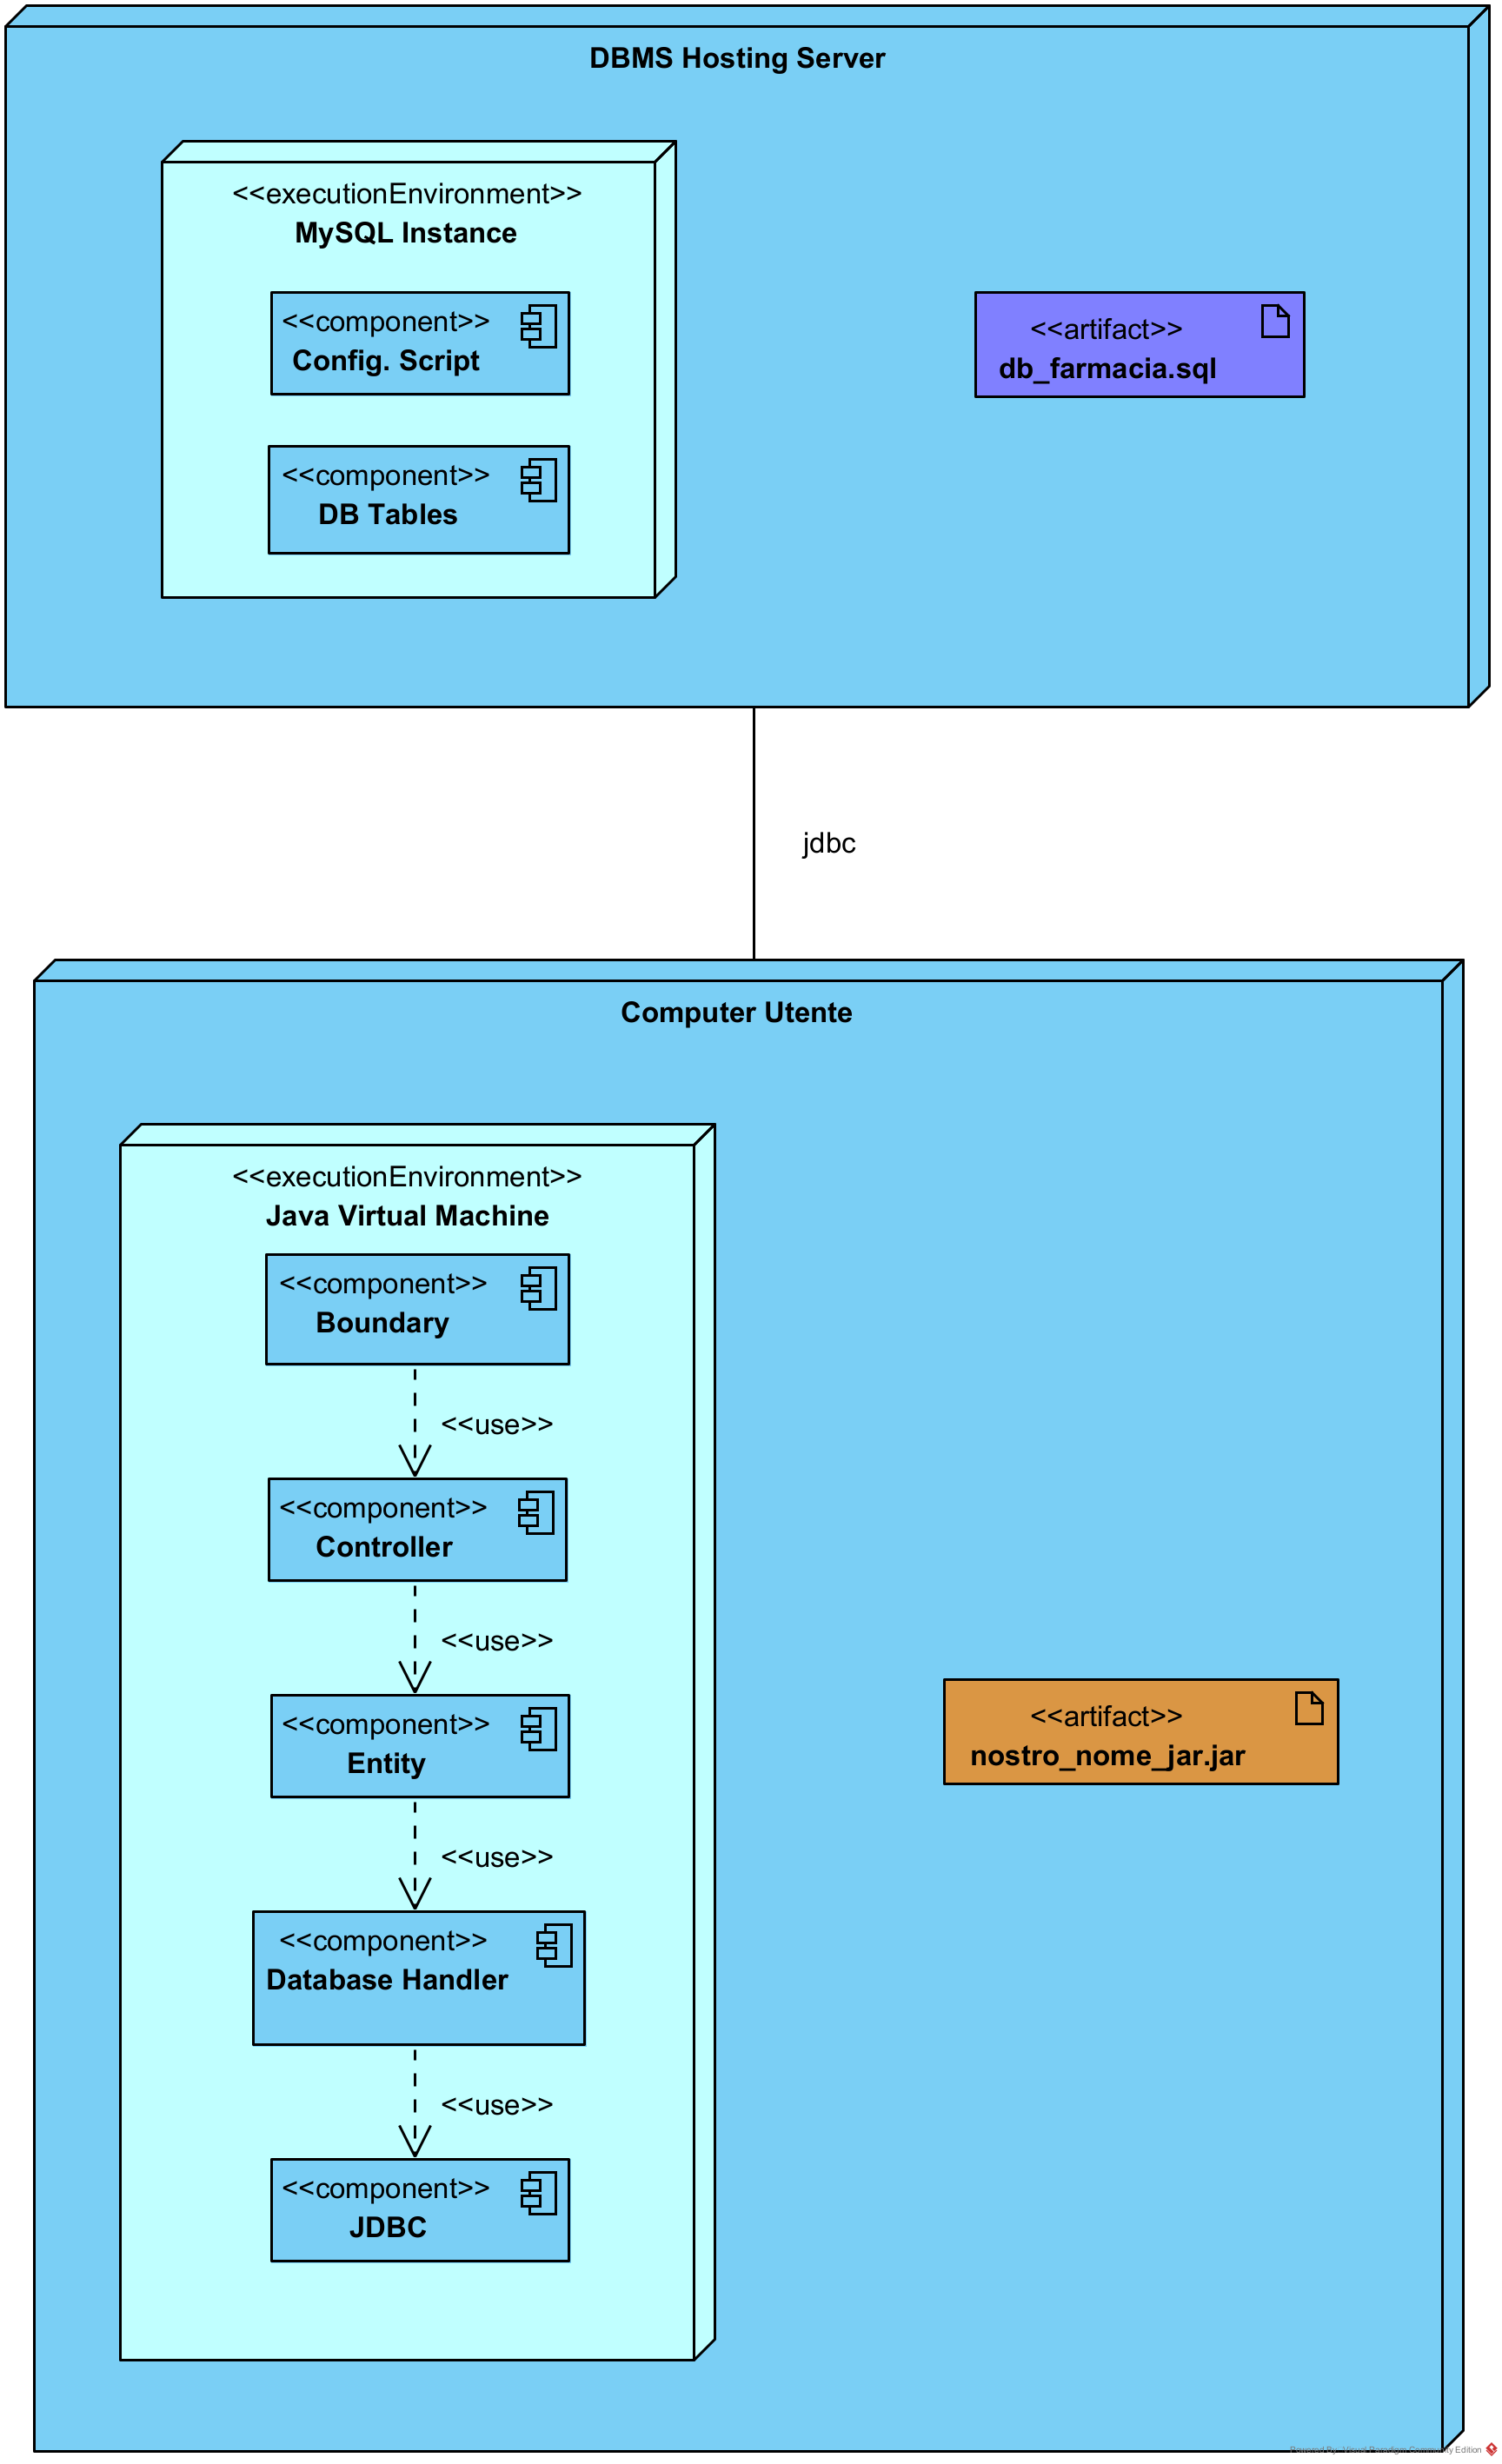
\includegraphics[width=0.65\textwidth]{assets/DeploymentFarmacia.png}
	\caption{Diagramma di deployment}
	\label{diag:deployment}
\end{figure}
